\documentclass[12pt]{article}
\usepackage[a4paper, hmargin={2.5cm, 2.5cm}, vmargin={2.5cm, 2.5cm}]{geometry}

\usepackage[utf8]{inputenc}
\usepackage[english]{babel}
\usepackage{amssymb}
\usepackage{amsfonts}
\usepackage{amsmath}
\usepackage{setspace}
\usepackage{algorithm}
\usepackage[noend]{algpseudocode}

\usepackage{tikz}
\usetikzlibrary{positioning,shapes, shadows, arrows, automata}

\usepackage{xcolor}
\usepackage{listings}
\usepackage{graphicx}
\usepackage[hidelinks]{hyperref}
\usepackage{float}
\usepackage[english]{varioref}
\usepackage{multirow}
\usepackage{hhline}
\usepackage{etoolbox}
\usepackage{tikz}

\usepackage{fancyhdr}

\setlength\parindent{0pt}
\usepackage[parfill]{parskip}

\definecolor{mygray}{rgb}{0.9451,0.9451,0.9451}
\lstset{
  backgroundcolor=\color{mygray},
  basicstyle=\footnotesize\ttfamily,
  mathescape,
  breaklines=true,
  numbers=left,
  numberstyle=\ttfamily,
  stepnumber=1,
  firstnumber=1,
  numberfirstline=true,
  postbreak=\raisebox{0ex}[0ex][0ex]{\ensuremath{\color{red}\hookrightarrow\space}},
  literate={->}{$\rightarrow$}{2}
           {ε}{$\varepsilon$}{1}
}

\linespread{1.3}

\title{
  \vspace{4cm}
  \begin{flushleft}
  \Large{\textbf{Mandatory Project 1}} \\
  \large{Computationally hard problems}
  \end{flushleft}
  \vspace{0cm}
  \begin{flushleft}
  \small
  \textit{\today}
  \end{flushleft}
  \vspace{12cm}
  \begin{flushleft}
  \small
  Troels Thomsen \texttt{152165} \\
  Rasmus Haarslev \texttt{152175}
  \end{flushleft}
}

\date{
	%
}

\begin{document}

\clearpage
\pagenumbering{gobble}
\thispagestyle{empty}
\maketitle

\newpage

\pagenumbering{arabic}

\section{Madragon}

\subsection{Determine whether the answer to the given Madragon instance is YES
or NO}
\label{sub:Determine whether the answer to the given Madragon instance is YES
or NO}

We take the following steps to shift the starting board to the goal board.

\textbf{Starting board}:


\begin{tikzpicture}
    \draw[step=1cm,black,thick] (0,0) grid (5,5);
    \fill[black] (0,0) rectangle (5,5);
    % col 1
    \fill[white] (0,3) rectangle (1,4);
    \fill[white] (0,2) rectangle (1,3);
    \fill[white] (0,1) rectangle (1,2);
    % col 2
    \fill[white] (1,3) rectangle (2,4);
    \fill[white] (1,1) rectangle (2,2);
    % col 3
    \fill[white] (2,4) rectangle (3,5);
    \fill[white] (2,2) rectangle (3,3);
    % col 4
    \fill[white] (3,3) rectangle (4,4);
    \fill[white] (3,1) rectangle (4,2);
\end{tikzpicture}

We move column 1 one tile up.

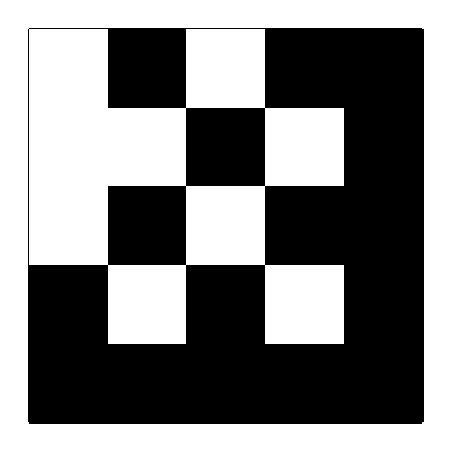
\begin{tikzpicture}
    \draw[step=1cm,black,thick] (0,0) grid (5,5);
    \fill[black] (0,0) rectangle (5,5);
    % col 1
    \fill[white] (0,4) rectangle (1,5);
    \fill[white] (0,3) rectangle (1,4);
    \fill[white] (0,2) rectangle (1,3);
    % col 2
    \fill[white] (1,3) rectangle (2,4);
    \fill[white] (1,1) rectangle (2,2);
    % col 3
    \fill[white] (2,4) rectangle (3,5);
    \fill[white] (2,2) rectangle (3,3);
    % col 4
    \fill[white] (3,3) rectangle (4,4);
    \fill[white] (3,1) rectangle (4,2);
\end{tikzpicture}

We column 2 two tiles down.


\begin{tikzpicture}
    \draw[step=1cm,black,very thick] (0,0) grid (5,5);
    \fill[black] (0,0) rectangle (5,5);
    % col 1
    \fill[white] (0,4) rectangle (1,5);
    \fill[white] (0,3) rectangle (1,4);
    \fill[white] (0,2) rectangle (1,3);
    % col 2
    \fill[white] (1,1) rectangle (2,2);
    \fill[white] (1,4) rectangle (2,5);
    % col 3
    \fill[white] (2,4) rectangle (3,5);
    \fill[white] (2,2) rectangle (3,3);
    % col 4
    \fill[white] (3,3) rectangle (4,4);
    \fill[white] (3,1) rectangle (4,2);
\end{tikzpicture}

We move row 3 two tiles to the left.


\begin{tikzpicture}
    \draw[step=1cm,black,very thick] (0,0) grid (5,5);
    \fill[black] (0,0) rectangle (5,5);
    % col 1
    \fill[white] (0,4) rectangle (1,5);
    \fill[white] (0,3) rectangle (1,4);
    \fill[white] (0,2) rectangle (1,3);
    % col 2
    \fill[white] (1,1) rectangle (2,2);
    \fill[white] (1,4) rectangle (2,5);
    % col 3
    \fill[white] (2,4) rectangle (3,5);
    \fill[white] (3,2) rectangle (4,3);
    % col 4
    \fill[white] (3,3) rectangle (4,4);
    \fill[white] (3,1) rectangle (4,2);
\end{tikzpicture}

And now we have made $k = 3$ operations and achieved the goal.

\subsection{Show that Madragon is in $NP$}
\label{sub:Show that Madragon is in NP}

We specify the following randomized deterministic polynomial-bound algorithm $A$, which takes as input a problem instance $X$ containing board states $a$ and $b$ and a random sequence of integers $R$.

\begin{enumerate}
    \item
        \begin{enumerate}
            \item[1a] $R$ is a random sequence of $k$ integers chosen from an even distribution of numbers ranging from 1 to $(m+n)\frac{(m-1)+(n-1)}{2}$.
            \item[1b] Every index in $R$ corresponds a step. The value of each index corresponds to a move of either a column or a row. Since there exists $(m+n)\frac{(m-1)+(n-1)}{2}$ unique moves, the value of $R_i$ will determine which of these moves the algorithm performs at the $i$th step.
            \item[1c] After $A$ has performed all $i$ steps in $R$, $A$ checks if the board has reached its goal state $b$ and answers YES or NO accordingly.
        \end{enumerate}
    \item
        \begin{enumerate}
            \item[2a] Since we choose $R$ from an evenly distributed set of all possible combinations of size $\{1, \cdots, (m+n)\frac{(m-1)+(n-1)}{2}\}^k = ((m+n)\frac{(m-1)+(n-1)}{2})^k$, we know that if at least one $R$ exists which solves $A(X, R) = YES$, we can choose this $R$ with a probability of $\frac{1}{((m+n)\frac{(m-1)+(n-1)}{2})^k} > 0$.
            \item[2b] If there does not exist an $R$ which solves $A(X, R) = YES$, then the algorithm $A$ will never answer YES since the board cannot arrive at goal board $b$ within $k$ steps given any $R$.
        \end{enumerate}
    \item
        In order to interpret $R$ the algorithm $A$ must generate all possible moves for the given board. This can be done in $O(((m+n)\frac{(m-1)+(n-1)}{2})^k)$ time. We can perform all steps in $R$ in $O(k)$ time, and check the solution in $O(1)$ time.
        Thus the algorithm is bound by $O(((m+n)\frac{(m-1)+(n-1)}{2})^k)$.
\end{enumerate}

\subsection{Show that Madragon is $NP$-complete}
\label{sub:Show that Madragon is $NP$-complete}

\begin{enumerate}
    \item
    In order to show that Madragon is $NP$-complete we must first show that the problem is in $NP$. Since we have shown this in section~\ref{sub:Show that Madragon is in NP} we can now choose a
    known $NP$-complete problem for the rest of our proof.

    \item
    For our proof we have chosen the $NP$-complete problem $P_c$ to be  \textit{LongestCommonSubsequence} or $LCS$. We will now show that $P_c \leq_p P$ where $P$ is the Madragon problem.
    We create the transformation $T$ for every instance of $X$ in $LCS$ into an instance of $P$ as follows.

    \item
    \begin{enumerate}
        \item[3a]
        In $LCS$ we have a set of words $W = \{w_1, w_2, \dots, w_n\}$ and a constant $B \leq |w_i|$ representing the length of the subsequence.
        We also have an implicit set $R$ containing all possible permutations of words of length $B$ chosen from alphabet $\Sigma_W = \{\forall x \in w | w \in W\}$ containing the set of letters in the words in $W$.

        We create a Madragon board where the number of columns equal the number of words $n = |W|$ and where the number of number of rows correspond to the size of $S$. We now mark all tiles in a row black if the permutation in $R$ corresponding to the given row index exists in all $w \in W$. As soon as we find one such row, we immediately mark all other rows entirely white. The Madragon board will now have zero or one row colored entirely black and all others entirely white. We choose this board as our starting board $a$.

        \begin{figure}[H]
            \begin{center}
                \begin{tabular}{|c|cccc|}
                    \hline
                    $x_{i,j} \in \Sigma_W$ & $w_1$ & $w_2$ & \cdots & $w_n$ \\
                    \hline
                    $\{x_{0,1}, \cdots, x_{0,k}\}$ & 0 & 0 & \cdots & 0 \\
                    \vdots & \enspace & \enspace & \vdots & \enspace \\
                    $\{x_{1,1}, \cdots, x_{1,k}\}$ & 1 & 1 & \cdots & 1 \\
                    \vdots & \enspace & \enspace & \vdots & \enspace \\
                    $\{x_{|R|,1}, \cdots, x_{|R|,k}\}$ & 0 & 0 & \cdots & 0 \\
                    \hline
                \end{tabular}
            \end{center}
            \caption{The board is represented here as 0s and 1s, where each 0 in
            the table corresponds to a white tile, and each 1 corresponds to a black tile.}
        \end{figure}

        We choose our final board $b$ as a board of equal size to $a$, but with only the top row colored entirely black. We choose our $k = n$.

        The time complexity of the transformation $T$ is bounded in the size of $B$ and $\Sigma_W$. This is due to the fact that $R$ must be of size $|R| = |\Sigma_W|^B$. Combining the size of $R$ with the fact that we can create the starting board $a$ in $O(n \times |R|)$, we get a total running time complexity of $O(|R|+n \times |R|) = O(n \times |R|) = O(|\Sigma_W|^B)$. As such the transformation $T$ is polynomially-bounded in $B$.

        \item[3b]
        If the answer to $LCS(X, B)$ is YES then the starting board $a$ will contain exactly one row with only black tiles. It will take at most $k = n$ moves to transform board $a$ into the final board $b$, since it takes $n$ steps to move any row up or down, using column moves, and there are $n$ total columns. Thus if the answer to $LCS(X, B)$ is YES, then the Madragon answer to $T(X)$ is also YES.

        \item[3c]
        Our final board $b$ in $T(X)$ looks the same no matter the given $LCS$ problem - it always contain the entire top row colored black with no other black tiles on the board. A starting board $a$ will never contain any black tiles if the answer to $LCS(X, B)$ is NO. Thus it is impossible for Madragon to answer YES to $T(X)$ if the answer to $LCS(X, B)$ is NO.

    \end{enumerate}

\end{enumerate}

\subsection{Describe the solution for the optimization version of the algorithm}
\label{sub:Describe the solution for the optimization version of the algorithm}

Our solution assumes, that for any given board $A$, there exists a set of moves $R_0$, such that $A$ may be transformed into any given board $B$, where $A$ and $B$ consists of the same number of black and white tiles.

Our optimization algorithm $A_o$ generates the set of possible moves $S = \{s_0, s_1, ...,s_n\}$ and the set $R = \{R_0, R_1, ..., R_m\}$, containing every combination of $k$-length move-sets from $S$.

We run all of the move-sets in $R$ against board $A$, and if one of the sets in $R$ transform board $A$ into goal board $B$, then the algorithm returns the move-set $R_0$, else $false$.

We run this process iteratively starting with $k = 1$ going up to $k = k_{max}$, where $k_{max}$ is the $k$ given in the .mad file.

\subsection{Prove the worst-case running time of your algorithm}
\label{sub:Prove the worst-case running time of your algorithm}

In the worst case, $A_o$ runs through all of the generated sets in $R$. Given that $R$ contains all possible permutations of $k_{max}$-length sets we have $|R| = |S|^{k_{max}} = ((m+n)\frac{(m-1)+(n-1)}{2})^{k_{max}}$ since $|S| = ((m+n)\frac{(m-1)+(n-1)}{2})^{k_{mx}}$. We can check each of these sets in $O(k_{max})$ time since each set is of length $k_{max}$ and each move can be performed in $O(1)$ constant time. Since we check all values of $k$ up to $k_{max}$, the algorithm is run $k_{max}$ times, but every time $k$ is incremented, the exponent in the calculation of permutation is incremented, which means the running time increases exponentially with $k$. This means that the running time of any iteration with $k < k_{max}$ does not matter in big-O notation.

This gives $A_o$ a worst-case running time of $T(A_o) = O(k|S|^k) = O(|S|^k)$.

\subsection{Implement the algorithm for Madragon}
\label{sub:Implement the algorithm for Madragon}

Out implementation can be run by running the file madragon:

\begin{lstlisting}
./madragon -f <path-to-file.mad>
\end{lstlisting}

Our implementation returns an array of the following format:

\begin{lstlisting}
[k, [
    [row / column, rotations], ..., ...]
]
\end{lstlisting}

Where $k$ is the $k$ for which a solution was found, and where $row / column$ is an integer representing which row or column to rotate.
If the number is less than the number of rows, we rotate the 0-indexed row in the number of rows on the board.
If the number is greater than or equal to the number of rows, we rotate the 0-indexed column in the number of columns on the board.

$rotations$ correspond to the number of times we rotate the given row or column. We always rotate from right to left or bottom to top.

For the file \textbf{arecibo-1.mad} the result would be:

\begin{lstlisting}
[1, [[8, 1]]]
\end{lstlisting}

Indicating that we can solve the board with a 1-length set of moves, and a move-set consisting of a single move where we rotating column 4 one step.

The source code for our implementation can be found on github: \url{https://github.com/ttsoftware/computationally-hard-problems/tree/master/group-project/code}

\end{document}
